\section{Pianificazione}
In questa sezione verrà riportata come l'attività di pianificazione del progetto è stata gestita dal gruppo Catch Em All. Il gruppo ha deciso di suddividere questa attività in vari periodi: 
\begin{itemize}
	\item \textbf{Analisi};
	\item \textbf{Sviluppo del Proof of Concept};
	\item \textbf{Progettazione architetturale};
    \item \textbf{Progettazione di dettaglio e Codifica};
	\item \textbf{Validazione\textsubscript{G} e Collaudo}.
\end{itemize}

\subsection{Analisi}
\subsubsection{Scopo}
Questo periodo ha lo scopo di analizzare in dettaglio il capitolato scelto dal gruppo in modo da definire i requisiti\textsubscript{G} funzionali, tempi e costi del progetto e gli obiettivi di qualità. Vengono anche definite in questo periodo le varie norme che il gruppo dovrà seguire per lavorare in modo efficacie ed efficiente.

\subsubsection{Periodo}
Il periodo di analisi inizierà con l'aggiudicazione del capitolato il 07/11/2022 e si svolgerà fino al completamento dei vari documenti necessari alla revisione  RTB. Il gruppo ha pianificato la fine di questo periodo per il 12/02/2023. Questo periodo sarà a sua volta suddiviso in vari sprint per ripartire in modo organizzato le attività che lo compongono.

\subsubsection{Ruoli attivi}
Durante il periodo di analisi saranno necessari i seguenti ruoli:
\begin{itemize}
	\item Responsabile;
	\item Amministratore;
	\item Analista;
	\item Verificatore.
\end{itemize}

\subsubsection{Sprint I}
\subsubsubsection{Scopo}
Lo scopo del primo sprint è quello di compiere una prima analisi del capitolato e impostare le prime norme e strumenti necessari che faranno da base al way of working del gruppo. Vengono inoltre redatti i primi verbali in modo da tenere traccia delle decisioni prese negli incontri interni e con il proponente.
\subsubsubsection{Durata}
Questo sprint si svolgerà nelle prime settimane di progetto. Inizierà il 07/11/2022 e terminerà il 27/11/2022.

\subsubsubsection{Precondizioni}\:
\begin{itemize}
	\item È stato formato il gruppo Catch Em All;
	\item È stato assegnato il capitolato d’appalto C1: \textit{CAPTCHA: umano o sovrumano?}.
\end{itemize}

\subsubsubsection{Postcondizioni}\:
\begin{itemize}
	\item Compiuta analisi preliminare del capitolato, seguita da uno studio di fattibilità sulle idee proposte dal gruppo;
	\item Scelti strumenti per la gestione dei compiti e ruoli dei vari membri;
	\item Scelta strumenti per la stesura dei documenti;
	\item Scrittura bozza dei documenti necessari alla revisione RTB;
	\item Fissata una base per il way of working del gruppo.
\end{itemize}

\subsubsubsection{Attività}\:
\begin{itemize}
	\item \textbf{Analisi preliminare fattibilità del capitolato}: Vengono discusse le varie proposte del gruppo per lo sviluppo del progetto, analizzandone pro e contro;
	\item \textbf{Ricerca degli strumenti}: Individuazione degli strumenti organizzativi e di supporto che saranno utilizzati durante il progetto per la suddivisione dei compiti e scrittura dei documenti;
	\item \textbf{Normazione}: Definizione delle norme alla base del way of working del gruppo, le quali sono illustrate nel documento \textit{Norme\_di\_progetto v 1.0.0};
    \item \textbf{Analisi dei requisiti}: Attività finalizzata alla comprensione dei bisogni espressi nel capitolato d’appalto e ricavati dallo studio del dominio\textsubscript{G} d’uso;
    \item \textbf{Analisi dei rischi}: Compiere una prima analisi dei rischi che il gruppo potrà incontrare nello sviluppo del progetto e fornire delle contromisure per evitare o ammortizzare i danni che questi possono causare.
\end{itemize}
\newpage
\subsubsection{Sprint II}\:
\subsubsubsection{Scopo}
Lo scopo del secondo sprint è quello di continuare l'analisi dei requisiti e dei casi d'uso del progetto, decidendo anche quali siano gli obiettivi di qualità che il progetto dovrà soddisfare. Vengono inoltre compiute una pianificazione e preventivo più dettagliate per la durata e i costi del progetto. In questo sprint il way of working del gruppo verrà migliorato in base ai riscontri ottenuti nel corso dello sprint precedente per avere un continuo miglioramento di efficienza ed efficacia nella completamento dei vari compiti assegnati ai membri.
\subsubsubsection{Durata}
Questo sprint seguirà le fasi iniziali del progetto. Inizierà il 28/11/2022 e terminerà il 25/12/2022.

\subsubsubsection{Precondizioni}\:
\begin{itemize}
	\item È stata svolta un analisi preliminare del capitolato;
	\item È stata impostata una base solida per il way of working del gruppo.
\end{itemize}

\subsubsubsection{Postcondizioni}\:
\begin{itemize}
	\item Definiti requisiti e casi d'uso necessari per il progetto, accompagnati dai vari obiettivi di qualità che dovranno essere rispettati;
	\item Pianificazione periodi e attività per l'intera durata del progetto;
	\item Fissate le varie norme che comporranno il way of working del gruppo.
\end{itemize}

\subsubsubsection{Attività}\:
\begin{itemize}
	\item \textbf{Normazione}: Definizione delle varie norme per i processi organizzativi e di supporto;
	\item \textbf{Obiettivi e metriche di qualità}: Individuazione degli obiettivi e metriche necessarie a garantire la qualità dei processi e dei prodotti per l'intera durata del progetto;
	\item \textbf{Analisi dei requisiti e casi d'uso}: Ricerca di tutti i requisiti e casi d'uso necessari per lo sviluppo del progetto;
	\item \textbf{Pianificazione periodi e attività}: Strutturare la pianificazione dei vari periodi del progetto fissando attività e obiettivi da raggiungere.
\end{itemize}

\subsubsection{Sprint III}
\subsubsubsection{Scopo}
Lo scopo del terzo sprint è quello di compiere una prima verifica completa delle attività svolte, e di conseguenza verificare che i vari documenti prodotti rispettino le norme definite e che i loro contenuti siano adeguati. In questo sprint viene inoltre svolta un'analisi sul way of working del gruppo, su come sia possibile migliorarlo e di come siano stati affrontati i vari imprevisti incontrati.
\subsubsubsection{Durata}
Questo sprint si svolgerà dopo la conclusione dell'analisi completa dei requisiti e casi d'uso del progetto e di una buona pianificazione di esso. Inizierà il 26/12/2022 e terminerà il 09/01/2023.

\subsubsubsection{Precondizioni}\:
\begin{itemize}
	\item È stato completata l'analisi dei requisiti e casi d'uso del progetto;
	\item I vari periodi e attività del progetto sono state definite.
\end{itemize}

\subsubsubsection{Postcondizioni}\:
\begin{itemize}
	\item Verifica della struttura e contenuti dei documenti prodotti;
	\item Compiuta analisi per il miglioramento del way of working sulle attività svolte.
\end{itemize}

\subsubsubsection{Attività}\:
\begin{itemize}
	\item \textbf{Normazione}: Aggiornamento delle norme in base ai riscontri e analisi svolte su attività completate;
	\item \textbf{Verifica}: Controllo qualità della struttura e contenuti dei documenti prodotti.
\end{itemize}

\subsubsection{Sprint V}
\subsubsubsection{Scopo}
Questo sprint è condiviso al periodo di \textit{Produzione del Proof of Concept}.
Lo scopo del quinto sprint per il periodo di \textit{Analisi} è quello di aggiornare i requisiti e casi d'uso del progetto a seguito dei riscontri ottenuti nelle attività di sviluppo del PoC.
\subsubsubsection{Durata}
Questo sprint si svolgerà parallelamente alle attività di sviluppo del PoC. Inizierà il 30/01/2023 e terminerà il 12/02/2023.

\subsubsubsection{Precondizioni}\:
\begin{itemize}
	\item È stata completata un'analisi delle tecnologie e della struttura del PoC;
	\item È stata impostata una base solida per lo sviluppo PoC.
\end{itemize}

\subsubsubsection{Postcondizioni}\:
\begin{itemize}
	\item Definiti in modo completo requisiti e casi d'uso del progetto;
	\item Definiti in modo chiaro obiettivi di qualità e test del sistema.
\end{itemize}

\subsubsubsection{Attività}\:
\begin{itemize}
	\item \textbf{Aggiornamento requisiti e casi d'uso}: Aggiornamento dei requisiti e casi d'uso in base ai riscontri ottenuti dallo sviluppo del PoC;
	\item \textbf{Miglioramento obiettivi di qualità}: Revisione e miglioramento degli obiettivi e metriche di qualità definite;
	\item \textbf{Test di sistema}: Definizione dei test di sistema che dovranno essere svolti sul prodotto finale.
\end{itemize}

\subsubsection{Sprint VI}
\subsubsubsection{Scopo}
Lo scopo del sesto sprint è quello di rilasciare i documenti necessari alla revisione RTB e verificare il Proof of Concept sviluppato. Il rilascio dovrà essere a carico del \textit{Re}.
\subsubsubsection{Durata}
Questo sprint si svolgerà a seguito del completamento del PoC e dei vari documenti necessari alla revisione RTB. Inizierà il 13/02/2023 e terminerà prima della revisione, pianificata per il 24/02/2023.

\subsubsubsection{Precondizioni}\:
\begin{itemize}
	\item È stato completato lo sviluppo del PoC;
	\item Sono stati completati tutti i documenti per la revisione RTB.
\end{itemize}

\subsubsubsection{Postcondizioni}\:
\begin{itemize}
	\item PoC e documenti sono stati rilasciati in versione 1.0.0;
	\item Completata la presentazione per la revisione RTB.
\end{itemize}

\subsubsubsection{Attività}\:
\begin{itemize}
	\item \textbf{Rilascio documenti}: Vengono verificati e rilasciati tutti i documenti per l'RTB. Il \textit{Re} si occuperà del loro rilascio;
	\item \textbf{Verifica e collaudo del PoC}: Il PoC sviluppato dovrà essere testato e collaudato per accertarsi che sia coerente con le aspettative e che gli obiettivi prefissati siano stati raggiunti;
	\item \textbf{Preparazione presentazione RTB}: Viene preparata la presentazione per la revisione RTB;
	\item \textbf{Lettera di candidatura}: Viene scritta la lettera che dichiara l'impegno del gruppo a candidarsi alla revisione RTB.
\end{itemize}

\subsubsection{Diagramma di Gantt\textsubscript{G} - Analisi}

\begin{figure}[H]
\centering
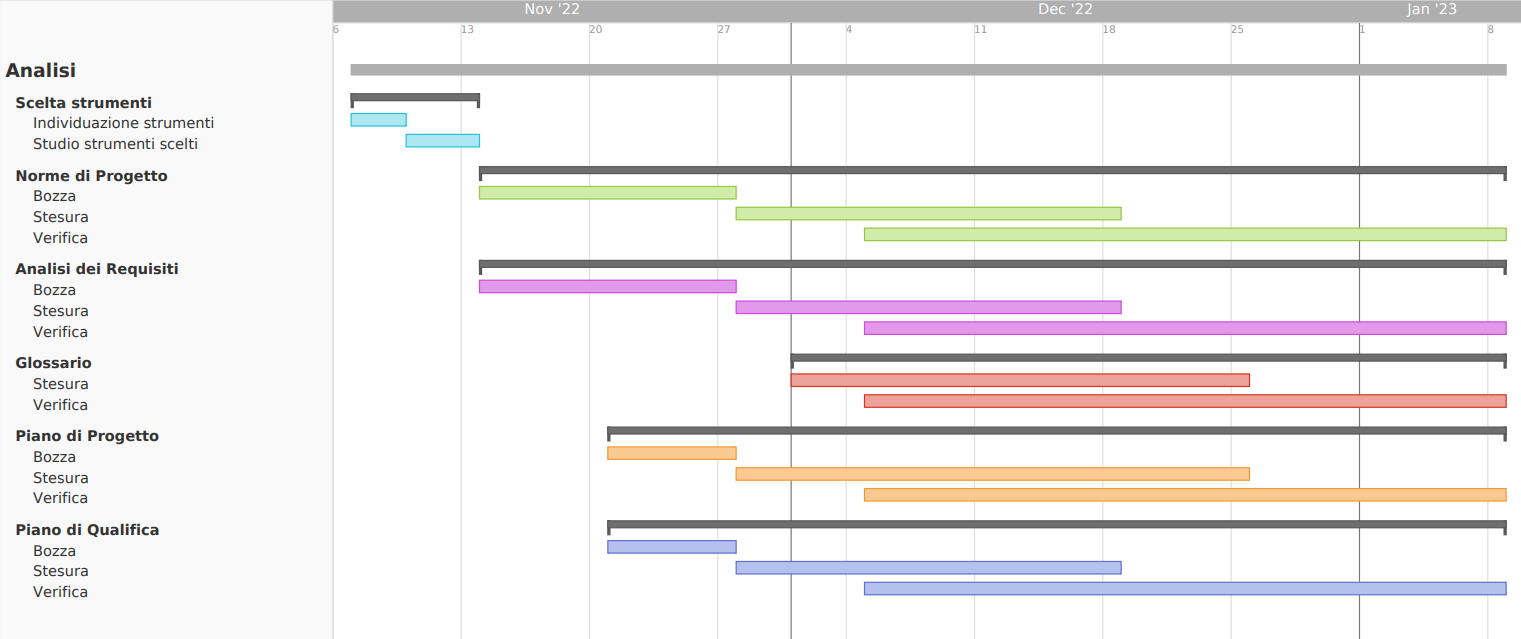
\includegraphics[width=\textwidth]{img/4_analisi.png}
\caption{Analisi}
\end{figure}

\subsection{Produzione del Proof of Concept}
\subsubsection{Scopo}
Lo scopo di questo periodo è quello di analizzare e scegliere la base tecnologica per il prodotto finale e quante di queste dovranno essere implementate nel \textit{PoC\textsubscript{G}}. In seguito a queste scelte si svolgerà l’attività di codifica del \textit{PoC\textsubscript{G}}.\\
La fase di produzione del Proof of Concept terminerà con la prima revisione \textit{RTB}.
\subsubsection{Periodo}
Il periodo di produzione del Proof of Concept inizierà dopo che il gruppo avrà svolto una solida analisi dei requisiti. L'inizio è pianificato per il 09/01/2023 e si svolgerà fino alla prima revisione di RTB, pianificata per 24/02/2023. Questo periodo sarà a sua volta suddiviso in 2 sprint per ripartire in modo organizzato le attività che lo compongono.

\subsubsection{Ruoli attivi}
Durante la fase di produzione del Proof of Concept saranno necessari i seguenti ruoli:
\begin{itemize}
	\item Responsabile;
    \item Amministratore;
    \item Analista;
    \item Progettista;
    \item Programmatore;
    \item Verificatore.
\end{itemize}

\subsubsection{Sprint IV}
\subsubsubsection{Scopo}
Lo scopo di questo sprint è quello di iniziare la realizzazione del Proof of Concept, scegliendo le tecnologie da utilizzare e seguito da uno studio approfondito su di esse.
\subsubsubsection{Durata}
Questo sprint avrà durata di tre settimane. Inizierà il 09/01/2023 e terminerà il 29/01/2023.

\subsubsubsection{Precondizioni}
I seguenti documenti sono stati redatti:
\begin{itemize}
	\item Norme di Progetto;
	\item Analisi dei Requisiti;
	\item Glossario;
    \item Piano di Progetto;
	\item Piano di Qualifica.
\end{itemize}

\subsubsubsection{Postcondizioni}\:
\begin{itemize}
	\item Determinate le tecnologie da utilizzare;
	\item I membri del gruppo hanno acquisito conoscenze sull'uso delle tecnologie scelte;
	\item Compiute scelte che saranno da base per la codifica del \textit{PoC\textsubscript{G}}.
\end{itemize}

\subsubsubsection{Attività}\:
\begin{itemize}
	\item \textbf{Individuazione requisiti\textsubscript{G} per il \textit{PoC\textsubscript{G}}}: Attività di analisi finalizzata all’individuazione dei requisiti\textsubscript{G} che il \textit{PoC\textsubscript{G}} andrà a soddisfare;
    \item \textbf{Progettazione Technology Baseline\textsubscript{G}}: Individuazione dell’architettura e delle tecnologie che saranno la base per l’implementazione del prodotto;
    \item \textbf{Approfondimento sulle tecnologie scelte}: I membri del gruppo si dedicano allo studio individuale delle tecnologie selezionate; al termine di questa attività tutti avranno acquisito le competenze necessarie per poter lavorare a rotazione sulla produzione del \textit{PoC\textsubscript{G}}.
\end{itemize}

\subsubsection{Sprint V}
\subsubsubsection{Scopo}
Questo sprint è condiviso al periodo di \textit{Analisi} per cui si svolgerà parallelamente alle attività di analisi. 
Lo scopo di questo sprint è la realizzazione effettiva del \textit{PoC\textsubscript{G}} utilizzando le tecnologie scelte nello sprint IV.
\subsubsubsection{Durata}
Questo sprint avrà durata di due settimane. Inizierà il 30/01/2023 e terminerà il 12/02/2023.

\subsubsubsection{Precondizioni}\:
\begin{itemize}
	\item Sono state determinate tecnologie da utilizzare per la realizzazione del \textit{PoC\textsubscript{G}};
	\item È stato fatto uno studio approfondito sulle tecnologie scelte.
\end{itemize}

\subsubsubsection{Postcondizioni}\:
\begin{itemize}
	\item E' stato sviluppato il \textit{PoC\textsubscript{G}};
	\item Il \textit{PoC\textsubscript{G}} è pronto per la verifica.
\end{itemize}

\subsubsubsection{Attività}\:
\begin{itemize}
    \item \textbf{Sviluppo della Technology Baseline\textsubscript{G}}: Attività di codifica del \textit{PoC\textsubscript{G}}.
\end{itemize}

\subsubsection{Diagramma di Gantt\textsubscript{G} - Produzione del Proof of Concept}

\begin{figure}[H]
\centering
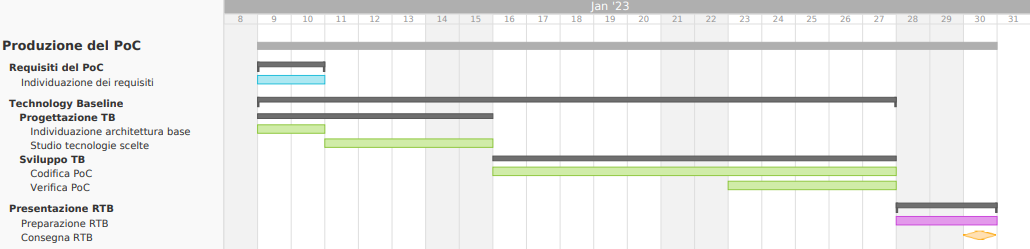
\includegraphics[width=\textwidth]{img/4_produzione.png}
\caption{Produzione del Proof of Concept}
\end{figure}

\subsection{Progettazione architetturale}
\subsubsection{Scopo}
Lo scopo di questo periodo è il raffinamento della progettazione architetturale ad alto livello avviata nel periodo di produzione del proof of concept, ovvero “come” saranno soddisfatti i requisiti\textsubscript{G} precedentemente individuati.
Le scelte che il gruppo effettua in questa fase riguarderanno la struttura complessiva del sistema e ne influenzeranno varie caratteristiche qualitative come per esempio l’efficienza, l’estensibilità e la manutenibilità.

\subsubsection{Periodo}
Il periodo di progettazione architetturale si svolgerà subito dopo la revisione \textit{RTB}. Il periodo va dal 27/02/2023 fino al 19/03/2023.\\
Questo periodo sarà svolto in un unico sprint.

\subsubsection{Ruoli attivi}
Durante la fase di progettazione architetturale saranno necessari i seguenti ruoli:
\begin{itemize}
	\item Responsabile;
    \item Amministratore;
    \item Analista;
    \item Progettista;
    \item Verificatore.
\end{itemize}

\subsubsection{Sprint VII}
\subsubsubsection{Scopo}
Lo scopo di questo sprint è quello di concludere la progettazione architetturale del prodotto.
\subsubsubsection{Durata}
Questo sprint avrà durata di tre settimane. Inizierà il 27/02/2023 e terminerà il 19/03/2023.

\subsubsubsection{Precondizioni}\:
\begin{itemize}
    \item È stato prodotto il \textit{PoC\textsubscript{G}};
    \item Superamento della prima revisione (\textit{RTB}).
\end{itemize}

\subsubsubsection{Postcondizioni}\:
\begin{itemize}
    \item Conclusione della progettazione architetturale ad alto livello.
\end{itemize}

\subsubsubsection{Attività}\:
\begin{itemize}
    \item \textbf{Incremento e verifica\textsubscript{G} dei documenti}: A seconda delle necessità, il gruppo si occupa di aggiornare la documentazione prodotta in precedenza;
    \item \textbf{Progettazione architetturale}: Raffinamento della progettazione architetturale ad alto livello;
        \subitem \textbf{Approfondimento sulle tecnologie scelte}: I membri del gruppo si dedicano allo studio individuale delle tecnologie selezionate; al termine di questa attività tutti avranno acquisito le competenze necessarie per poter lavorare a rotazione sulla futura realizzazione del prodotto.
\end{itemize}

\subsubsection{Diagramma di Gantt\textsubscript{G} - Progettazione architetturale}

\begin{figure}[H]
\centering
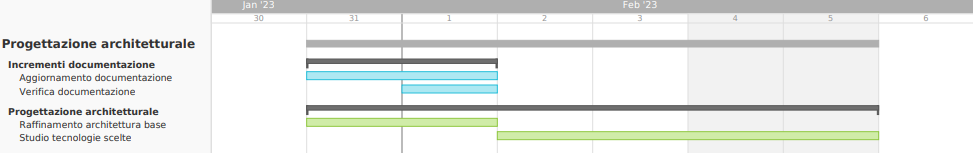
\includegraphics[width=\textwidth]{img/4_progettazione.png}
\caption{Progettazione architetturale}
\end{figure}

\subsection{Progettazione di dettaglio e codifica}
\subsubsection{Scopo}
Questo periodo ha lo scopo di avviare le attività riguardanti la progettazione di dettaglio del sistema e la codifica del prodotto.
In particolare, la codifica si svolgerà in base alle norme di codifica stabilite nel documento \textit{Norme di Progetto} e avrà tra gli obiettivi anche l’assicurarsi di scrivere codice facilmente verificabile in modo da facilitare le attività di validazione e collaudo. Questo in quanto l'efficacia dei metodi di verifica\textsubscript{G} è strettamente legata alla qualità di strutturazione del codice. In questo modo non sarà necessario dipendere solo dalla verifica\textsubscript{G} retrospettiva, il cui costo cresce con l'avanzare della fase di codifica.

\subsubsection{Periodo}
La fase di progettazione di dettaglio e codifica inizierà quando il gruppo avrà completato la progettazione architetturale del prodotto. L'inizio è pianificato per il 20/03/2023 e durerà fino al 23/04/2023.

\subsubsection{Ruoli attivi}
Durante la fase di progettazione di dettaglio e codifica saranno necessari i seguenti ruoli:
\begin{itemize}
	\item Responsabile;
	\item Amministratore;
	\item Progettista;
	\item Programmatore;
	\item Verificatore.
\end{itemize}

\subsubsection{Sprint VIII}
\subsubsubsection{Scopo}
Lo scopo dell'ottavo sprint è quello di concludere la progettazione di dettaglio del prodotto e iniziare la stesura dell’Allegato tecnico. Questo sprint ha lo scopo di porre tutte le basi necessarie all'inizio delle attività di codifica.
\subsubsubsection{Durata}
Questo sprint inizierà con la conclusione delle attività di progettazione architetturale. Inizierà il 20/03/2023 e terminerà il 02/04/2023.

\subsubsubsection{Precondizioni}\:
\begin{itemize}
	\item Il gruppo ha concluso la progettazione architetturale del prodotto.
\end{itemize}

\subsubsubsection{Postcondizioni}\:
\begin{itemize}
	\item Conclusa la progettazione di dettaglio del prodotto;
	\item Definite tutte le norme da seguire durante le attività di codifica;
	\item Definiti i test di unità del prodotto.
\end{itemize}

\subsubsubsection{Attività}\:
\begin{itemize}
	\item \textbf{Product Baseline}: Attività nella quale vengono studiati i vari design pattern da utilizzare e implementati nei vari diagrammi delle classi e di sequenza del prodotto;
	\subitem \textbf{Definizione delle unità software\textsubscript{G} che comporranno il prodotto}: Il prodotto viene suddiviso in unità, ciascuna delle quali potrà essere realizzata da un singolo programmatore;
	\item \textbf{Normazione}: Vengono definite in modo chiaro e dettagliato tutte le norme necessarie alla codifica del prodotto;
	\item \textbf{Stesura dell’allegato tecnico}: Viene scritto il documento che descrive le caratteristiche architetturali del prodotto in base alle scelte fatte dal gruppo;
	\item \textbf{Obiettivi di qualità}: Vengono aggiornati se necessario gli obiettivi e metriche di qualità del prodotto definite;
	\item \textbf{Test di unità}: Vengono definiti i test di unità da svolgere sui singoli moduli del prodotto;
	\item \textbf{Pianificazione}: Vengono aggiornate le attività e i preventivi del progetto se necessario.
\end{itemize}

\subsubsection{Sprint IX}
\subsubsubsection{Scopo}
Lo scopo del nono sprint è quello di svolgere le attività di codifica e verifica per lo sviluppo delle componenti che coprono i requisiti obbligatori 
del prodotto, seguendo le decisioni prese durante il periodo di progettazione e le norme fissate.
\subsubsubsection{Durata}
Questo sprint si svolgerà a seguito della definizione della product baseline e con la conclusione della progettazione di dettaglio. Inizierà il 03/04/2023 e terminerà il 16/04/2023.

\subsubsubsection{Precondizioni}\:
\begin{itemize}
	\item Il gruppo ha concluso la progettazione di dettaglio del prodotto.
\end{itemize}

\subsubsubsection{Postcondizioni}\:
\begin{itemize}
	\item Conclusa la codifica delle componenti riguardanti i requisiti obbligatori del prodotto in modo coerente con quanto definito nel periodo di progettazione.
\end{itemize}

\subsubsubsection{Attività}\:
\begin{itemize}
	\item \textbf{Codifica}: Utilizzando il \textit{PoC\textsubscript{G}} prodotto in precedenza e la product baseline definita durante la progettazione di dettaglio, viene prodotto il codice per lo sviluppo delle componenti riguardanti i requisiti obbligatori del prodotto. La codifica avverrà utilizzando un approccio incrementale, per cui ogni incremento sarà costituito dalla codifica di un determinato caso d’uso e produrrà valore aggiunto;
	\subitem \textbf{Verifica\textsubscript{G}}: Il codice prodotto viene continuamente verificato, tramite i test di integrazione e di unità definiti nel \textit{Piano di qualifica}. Questa attività prepara il successo della fase di validazione\textsubscript{G}.
\end{itemize}

\subsubsection{Sprint X}
\subsubsubsection{Scopo}
Lo scopo del decimo sprint è quello di codificare e verificare i requisiti opzionali. Nel corso di questo sprint devono anche essere prodotti il manuale utente e di manutenzione del prodotto.
\subsubsubsection{Durata}
Questo sprint si svolgerà a seguito della fase di codifica e verifica dei requisiti obbligatori. Inizierà il 17/04/2023 e terminerà il 24/04/2023.

\subsubsubsection{Precondizioni}\:
\begin{itemize}
	\item Il gruppo ha concluso la codifica e verifica dei requisiti obbligatori.
\end{itemize}

\subsubsubsection{Postcondizioni}\:
\begin{itemize}
	\item Conclusa la codifica del prodotto soddisfando tutti i requisiti obbligatori e opzionali in modo coerente con quanto definito nel periodo di progettazione;
	\item Prodotti manuali utente e di manutenzione;

\end{itemize}

\subsubsubsection{Attività}\:
\begin{itemize}
	\item \textbf{Codifica} Partendo dall'artefatto prodotto al periodo precedente si codificano i requisiti opzionali in modo incrementale;
	\subitem \textbf{Verifica\textsubscript{G}}: Il codice prodotto viene continuamente verificato, tramite i test di integrazione e di unità definiti nel \textit{Piano di qualifica}. Questa attività prepara il successo della fase di validazione\textsubscript{G};
	\item \textbf{Stesura del manuale per la manutenzione del prodotto}: Viene prodotto il manuale per la manutenzione e le estensioni future del prodotto;
	\item \textbf{Stesura del manuale utente}: Viene prodotto il manuale contenente le istruzioni di utilizzo del prodotto.
\end{itemize}
\subsubsection{Diagramma di Gantt\textsubscript{G} - Progettazione di dettaglio e Codifica}

\begin{figure}[H]
\centering
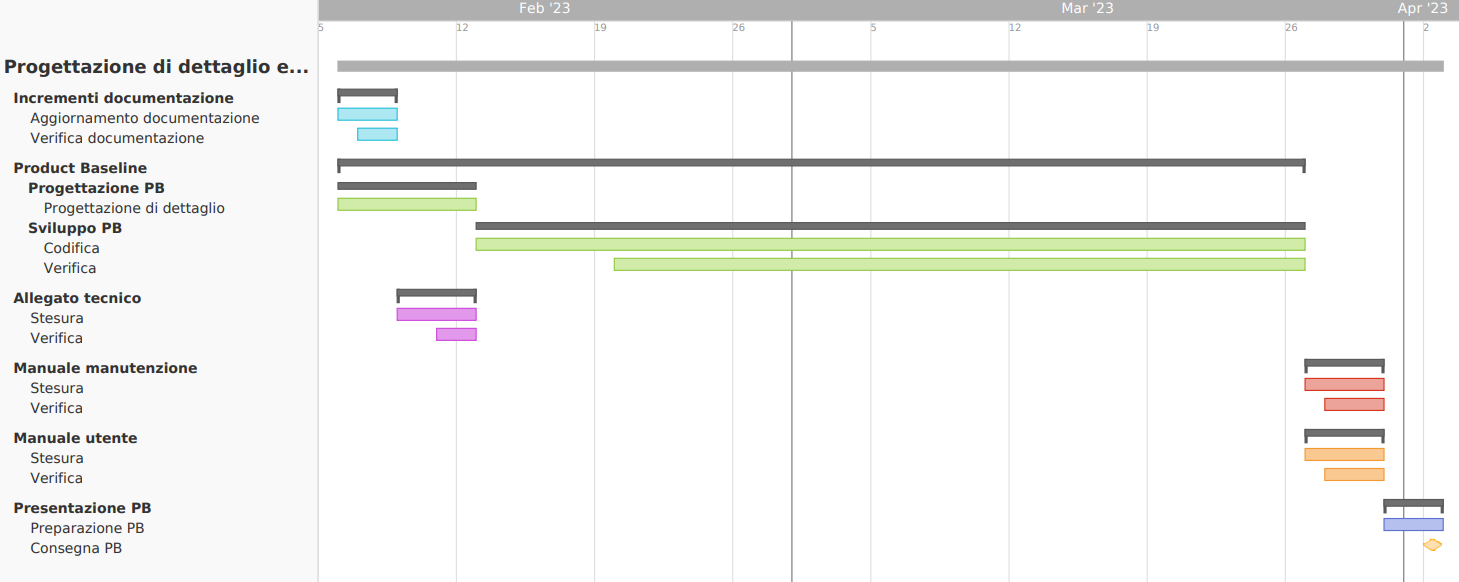
\includegraphics[width=\textwidth]{img/4_codifica.png}
\caption{Progettazione di dettaglio e Codifica}
\end{figure}

\newpage
\subsection{Validazione\textsubscript{G} e Collaudo}
In questo periodo vengono effettuati i controlli per garantire che il prodotto finale soddisfi le attese degli stakeholder. Il progetto si concluderà con la validazione\textsubscript{G} del prodotto, verificando che il sistema sia completo e funzionale rispetto ai requisiti\textsubscript{G} stabiliti nei periodi precedenti.

\subsubsection{Periodo}
Il periodo di validazione e collaudo si svolgerà con la conclusione della codifica del prodotto. Inizierà il 25/04/2023 e terminerà il 07/05/2023.

\subsubsection{Ruoli attivi}
Durante la fase di validazione\textsubscript{G} e Collaudo saranno necessari i seguenti ruoli:
\begin{itemize}
	\item Responsabile;
	\item Amministratore;
	\item Programmatore;
	\item Verificatore.
\end{itemize}

\subsubsection{Sprint XI}
\subsubsubsection{Scopo}
Lo scopo dell'undicesimo sprint è quello di validare i documenti necessari alla revisione PB e collaudare il MVP sviluppato. A seguito della validazione il \textit{Re} dovrà dare il consenso al rilascio dei prodotti.
\subsubsubsection{Durata}
Questo sprint si svolgerà a seguito del completamento delle attività di codifica e verifica e della produzione dei manuali utente e di manutenzione del prodotto. Il suo inizio è pianificato per il 25/04/2023 e terminerà prima della revisione PB, pianificata per il 07/05/2023.

\subsubsubsection{Precondizioni}\:
\begin{itemize}
	\item È stato completato lo sviluppo del MVP;
	\item Sono stati prodotti i manuali utente e di manutenzione del prodotto.
\end{itemize}

\subsubsubsection{Postcondizioni}\:
\begin{itemize}
	\item Il MVP è stato validato e collaudato;
	\item I documenti sono stati rilasciati nella loro versione finale;
	\item Completata la presentazione per la revisione PB.
\end{itemize}

\subsubsubsection{Attività}\:
\begin{itemize}
	\item \textbf{Validazione documenti}: Vengono validati tutti i documenti per la revisione PB. Il \textit{Re} si occuperà del loro rilascio;
	\item \textbf{Validazione e collaudo del MVP}: Il MVP sviluppato dovrà superare tutti i test di sistema definiti nel \textit{Piano di qualifica}. Il gruppo dovrà anche accertarsi che esso sia coerente con le aspettative e che gli obiettivi di qualità fissati;
	\item \textbf{Preparazione presentazione PB}: Viene preparata la presentazione per la revisione PB;
	\item \textbf{Lettera di candidatura}: Viene scritta la lettera che dichiara l'impegno del gruppo a candidarsi alla revisione PB.
\end{itemize}

\subsubsection{Diagramma di Gantt\textsubscript{G} - validazione\textsubscript{G} e Collaudo}

\begin{figure}[H]
\centering
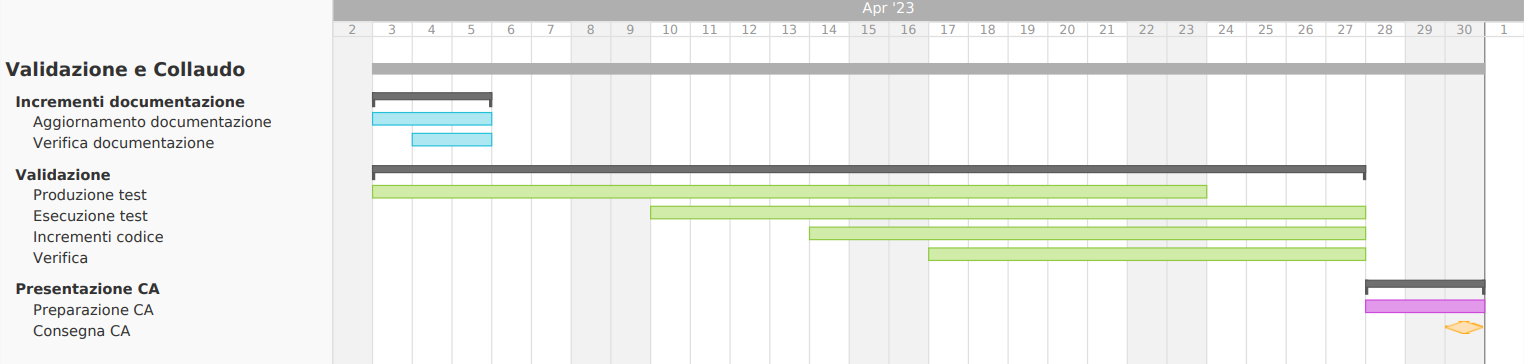
\includegraphics[width=\textwidth]{img/4_collaudo.png}
\caption{validazione\textsubscript{G} e Collaudo}
\end{figure}

